% 这个文件是用来定义其他 Latex 文档基本的、通用的样式的
% 中文文档
\documentclass{ctexart}

% 使用超链接宏包
\usepackage{hyperref}
% 设置纸张的宏包
\usepackage{geometry}
% 用于绘图的宏包
\usepackage{tikz}
% 用于书写数学公式的宏包
\usepackage{amsmath}
% 用户设置字体的宏包
\usepackage{fontspec}

% 定义纸张大小为 A4,内容所占区域为 95%
\geometry{a4paper, scale=0.95}
% 定义超链接样式
\hypersetup{
    CJKbookmarks=true, % 支持中文书签
    colorlinks=true,
    citecolor=blue,
    linkcolor=blue,
    urlcolor=blue,
    breaklinks=true % 允许链接中的换行
}

% 设置字体
% 设置英文字体
\setmainfont{JetBrains Mono}
% 设置中文字体
\setCJKmainfont{130-SS Zhui Guang Shou Xie Ti}

%作者
\author{aszswaz}


\usepackage{../latex-packages/axis}

\title{数学-名词定义}
\date{2022-03-22}

\begin{document}
% 生成标题
\maketitle\clearpage
% 生成目录
\tableofcontents

\clearpage
% 微积分学名词定义
\section{微积分学}

\subsection{\href{https://zh.wikipedia.org/wiki/\%E5\%AF\%BC\%E6\%95\%B0}{导数}}
\subsubsection{导数的定义}
\textbf{导数}(英语:derivative)是微积分学中的一个概念。函数在某一点的导数是指这个函数在这一点附近的变化率。导数的本质是通过极限的概念对函数进行局部的线性逼近。

导数是函数的局部性质。导数实际上是函数的切线的斜率,如图所示:

\begin{center}
	\begin{tikzpicture}
		% 画函数抛物线
		\draw (0, 0) .. controls (1, 1) and (2, 1) .. (3, 0);
		\draw (3, 0) .. controls (4, -1) and (5, -1) .. (6, 0);
		% 化函数抛物线的切线
		\draw[green] (0, 1.38) -- (6, -0.73);
		\filldraw[black] (2, 0.66) circle (1 pt);
	\end{tikzpicture}
\end{center}

实际上这条切线是两个距离非常小的端点,确定的一条直线:

% 函数中的导数示意图
\begin{center}
	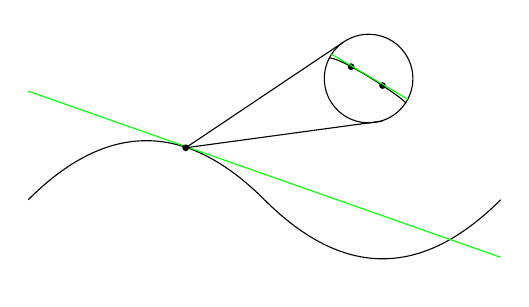
\begin{tikzpicture}
		% 画函数抛物线,以及抛物线的切线
		\draw (0, 0) .. controls (1, 1) and (2, 1) .. (3, 0);
		\draw (3, 0) .. controls (4, -1) and (5, -1) .. (6, 0);
		\draw[green] (0, 1.38) -- (6, -0.73);
		\filldraw[black] (2, 0.66) circle (1 pt);

		% 画函数局部放大图
		\draw (2, 0.66) -- (4, 2);
		\draw (2, 0.66) -- (4.5, 1);
		\draw (4, 2) arc (125:485:0.5625);
		\draw (3.825, 1.8) .. controls (4, 1.8) and (4.75, 1.3) .. (4.80, 1.225);
		\filldraw[black] (4.1, 1.69) circle (1 pt);
		\filldraw[black] (4.5, 1.45) circle (1 pt);
		\draw[green] (3.85, 1.85) -- (4.825, 1.275);
	\end{tikzpicture}
\end{center}

两个端点之间的线段,在距离非常小的情况下,也只是近似直线,但是实际上也还是存在一定的弧度。套用一个 B 站 UP 主的一句话:“这种直是宏观的“弯曲”在微观中的一种近似。”\\
假设两个端点的坐标分别为 $(x_0, y_0)$ 和 $(x_1, y_1)$,那么 $\Delta x = x_1 - x_0$($\Delta$ 表示改变量),$\Delta y = y_1 - y_0$,那么斜率 $K = \frac{\Delta y}{\Delta x}$。

% 通过直线,表示导数
\begin{center}
	\begin{tikzpicture}[
			nodefont/.style={font=\fontsize{6}{6}\selectfont}
		]
		% 画两个端点和穿过两个端点的直线
		\filldraw (1, 1) circle (1 pt) node[nodefont] at(1, 0.7) {$(x_0, y_0)$};
		\filldraw (4, 5) circle (1 pt) node[nodefont] at(4, 4.5) {$(x_1, y_1)$};
		\draw (0.25, 0) -- (5, 6.33);

		% 两个端点的垂直线和水平线的焦点
		\draw[dashed, thick] (1, 1) -- (4, 1) -- (4, 5);
		\draw node[nodefont] at(5, 3.125) {$\Delta y = y_1 - y_0$};
		\draw node[nodefont] at(2.5, 1.25) {$\Delta x = x_1 - x_0$};
	\end{tikzpicture}
\end{center}

\textbf{导数的符号}:$f$ 在 $x_0$ 处的导数,记作 $f'(x_0)$、$\frac{\mathrm{d}f}{\mathrm{d}x}$ 或 $\frac{\mathrm{d}f}{\mathrm{d}x}|_{x=x_0}$

\subsubsection{导数的求导法则}
\begin{enumerate}
	\item \textbf{定义法},假设函数 $f(x) = x^2$,那么它在 $x_0$ 处的导数 $f'(x)$ 的求导过程为:

	      \[
		      \begin{aligned}
			      f'(x) & = \lim_{x \to 0} \frac {f(x + \Delta x) - f(x_0)}{\Delta x} \\
			            & = \lim_{x \to 0} \frac {(x + \Delta x)^2 - x^2}{\Delta x}   \\
			            & = \lim_{x \to 0} \frac {\Delta x^2 + 2x \Delta x}{\Delta x} \\
			            & = \lim_{x \to 0} (\Delta x + 2x)                            \\
			            & = 2x
		      \end{aligned}
	      \]

	      注意 $\lim_{x \to 0} (\Delta x + 2x)$,当 $\Delta x$ 无穷小的时候,$\Delta x$ 就会湮灭,也可以理解为此时的 $\Delta x = 0$。

	\item \textbf{乘积法则}(英语:Product rule),也称积定则、莱布尼兹法则,是数学中关于两个函数的积的导数的一个计算法则。

	      若已知两个可导函数 $f'$、$g'$,则他们的积 $fg$ 的导数为:$(fg)' = f'g + fg'$。
\end{enumerate}

\subsubsection{导数的特性}

\begin{enumerate}
	\item 常数函数的导数永远都是 0。
	\item 幂函数的导数是把幂放到前面,再把幂减 1:$f'(x^a) = ax^{a-1}$。
	\item 一元二次函数 $ax^2 + bx + c$ 的导数为:$K = 2aw + b$。
\end{enumerate}

\clearpage
\subsection{函数}

\subsubsection{\href{https://zh.wikipedia.org/wiki/\%E5\%B8\%B8\%E6\%95\%B8\%E5\%87\%BD\%E6\%95\%B8}{常数函数}}

\textbf{常数函数}又叫常函数、常值函数,是指值不发生改变的函数。比如,函数 $f(x) = 4$,因为 $f$ 映射任意的值到 4,因此 $f$ 是一个常数。对一个函数:$f: A \rightarrow B$,如果对 $A$ 内所有的 $x$ 和 $y$,都有 $f(x) = f(y)$,那么 $f$ 是一个常数函数。其中 $f(x) = 0$ 是零函数。

\subsubsection{\href{https://zh.wikipedia.org/wiki/\%E5\%B9\%82\%E5\%87\%BD\%E6\%95\%B0}{幂函数}}

\textbf{幂函数}(英语:Power function)是形如 $f(x) = x^a$ 的函数,$a$ 可以是自然数、有理数,也可以是任意实数或复数。

\end{document}
